\documentclass[a4paper, 11pt]{article}
\usepackage[margin=2cm]{geometry}
\usepackage{graphicx}
\usepackage{hyperref}
\usepackage{amsmath}
\usepackage{amssymb}

\title{\textbf{COMP90056 Assignment A Report}}
\author{Tingsheng (Tinson) Lai (731319)}
\date{2019}

\begin{document}
    \maketitle
    \section{Introduction}
    Count-Min Sketch is an introductory technique used in stream computing. Specifically, it is a probabilistic data structure for frequency counting returning a (potentially) accurate estimate. Traditionally, the well-known basic technique used for frequency counting is the hash table. It has comparatively fastest update and query process, and it always produces exact results. The only problem is that it needs to record the identities of all items in the stream of data to resolve problems incurred by collisions of hashes. This is considered to be a waste of space as we are not interested in the actual identities. This report will briefly examine the techniques introduced by the Count-Min Sketch to tackle the issues caused by randomness and how it can minimise the effect of hash collisions.
    \section{Theory}
        To start with, the standard Count-Min Sketch draws multiple hash functions from a hash family uniformly at random, and the number of hash functions is denoted as $d$. Intuitively, this introduces randomness, and it decreases the probability of collisions for pairs of items in the stream. Correspondingly, the item will be hashed to the same number of different positions in a matrix, and the update will be applied to these $d$ cells. Essentially, this matrix can be viewed as multiple counters with a fixed width. By definition, the frequency of an item $x$, defined as the sum of all updates, will always be non-negative. Even if the item collides with another item in the stream, the total frequency will never be less than the original individual frequency. Hence, we claim this data structure will always overestimate the frequency of a given item. \\

        \noindent The conservative variant avoids stacking multiple updates due to collisions. The trade-off is to double the runtime compared to the default version. \\

        \noindent The morris counter variant dramatically reduces the memory usage, but we expect to see a dropdown of accuracy for querying. It may underestimate some of the frequencies due to the randomness introduced in the update. \\

        \noindent We can summarise the theoretical complexity in the following table. $d$ and $w$ are two parameters derived from $\epsilon$ and $\delta$ where $d = \log_{2}{\frac{1}{\delta}}$ and $w = \frac{2}{\epsilon}$. $n$ is the size of the universe. Another assumption used in the table is that the random generator will yield a random number with time complexity of $O(1)$.
        \begin{table}[!h]
            \centering
            \begin{tabular}{|c|c|c|c|}
                \hline
                                     & \textbf{Standard} & \textbf{Conservative Update} & \textbf{Morris Counter} \\
                \hline
                \textbf{Memory}      & $O(dw\ln{n})$     & $O(dw\ln{n})$                & $O(dw\ln{\ln{n}})$      \\
                \hline
                \textbf{Update Time} & $O(d)$            & $O(d)$                       & $O(d)$                  \\
                \hline
                \textbf{Query Time}  & $O(d)$            & $O(d)$                       & $O(d)$                  \\
                \hline
            \end{tabular}
            \caption{Comparison of different implementations}
            \label{table:comparison}
        \end{table}
    \section{Implementation}
        The assignment was entirely implemented in C++17 as C++ provides sophisticated memory control, and we can get a more accurate estimate of the measurement of memory usage programmatically. The reason for it to be an accurate estimate instead of the exact result is that there are other negligible factors which may slightly increase the actual memory usage, such as alignment of data types. This is better than measuring the runtime memory directly as other significant factors, such as concurrent executions or memory management techniques, will affect the result severely. The hash functions are simply drawn from the 2-universal hash family. \\

        \noindent One minor issue here is that it may not have the property of strong universality as two random variables share the same random number engine, Mersenne Twister generator, provided in the C++ Standard Template Library. I implemented this deliberately to boost the execution, and also it will be more similar to the random number generator in the provided stdlib.jar file for Java. This issue is almost irresolvable as most of the provided random number generators always use some forms of pseudo-random generation algorithm. Maybe we can consider using the random number generation API from random.org which claims to use the atmospheric noises to generate the random numbers. \\

        \noindent In the actual implementation, I used fixed-width integer type definitions to force the size of the data types to be the same across platforms. I also chose the data type with as smallest size as possible. Some of the data types chosen in the stream are based on the consideration of avoiding unintentional integer overflow. \\

        \noindent The Count-Min Sketch variant with Morris counter is the most interesting implementation amongst all three implementations. The implementation is separately designed leveraging the power of the technique of template partial specialisation, and they can adapt to different models of stream, specifically, the cash-register model and turnstile model. To tackle the negative update in the turnstile stream, I introduced an extra counter for negative updates, whereas the normal counter (inherited from the base class) will only be used for positive updates. The consequence is double the space needed, but it is still far less than the Count-Min Sketch using regular numbers as counters. The query will subtract the negative counter from the positive counter and return the resulting value. It implies $E \left[ Y_{\text{result}} \right] = E \left[ Y_{\text{pos}} - Y_{\text{neg}} \right] = E \left[ Y_{\text{pos}} \right] - E \left[ Y_{\text{neg}} \right]$, so we can conclude that the resulting value $Y_{\text{result}}$ is a reasonable estimate based on the fact that $Y_{\text{pos}}$ and $Y_{\text{neg}}$ are good estimates.
    \section{Experimental Set Up}
        As the technique of hash table is applied widely in the field of computer science and software engineering, it is well-known that the amortised time complexity of query and update in hash tables is $O(1)$ though some expensive operations such as rehashing and expansions may occur during insertion. I only focus on the memory used by hash table. \\

        \noindent There was a stream generator which can generate item with string type\footnote{\url{https://github.com/laitingsheng/COMP90056/blob/2ebab4b1699690457c181989a10755cfe9b7cb28/Assignment/Assignment1/stream.hpp} (This repository is just a mirror of my original repository on GitLab. Only master branch will be synced to this repository.)}. But I deleted this after a reconstruct of the stream runner class since the memory usage will be very intensive when the scale of data stream grows to a very large size. The current encapsulation is flexible to accommodate more distributions and data types. \\

        The experiment is done to compare different combinations of $\epsilon$s, $\delta$s and the numbers of distinct items in the stream. It will be executed for 16 times to provide more rigorous results.
    \section{Results \& Discussion}
        One of the weird result is that the accuracy for most of the results are 100\%. One of the possible reasons is that the first frequency moment $F1$ is comparatively much larger than any individual frequency. We can see this from the extrema of the ratios. \\

        \noindent The morris counter variants, as expected, will sometimes underestimate the frequency. It is also noticeable that the memory for turnstile stream is indeed double the original size.

        \begin{center}
            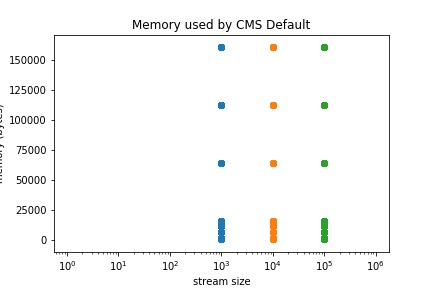
\includegraphics[scale=0.5]{memory_default}
            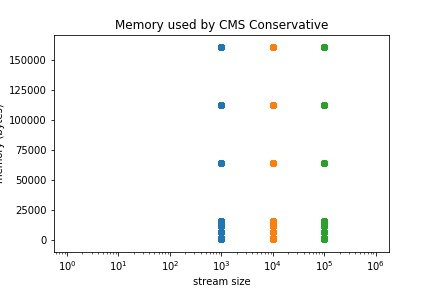
\includegraphics[scale=0.5]{memory_conservative}
        \end{center}

        \begin{center}
            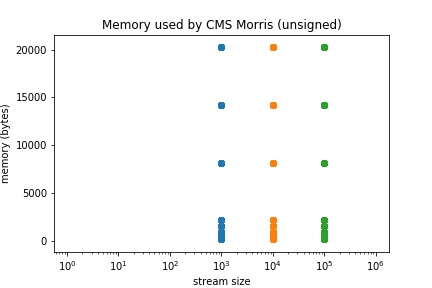
\includegraphics[scale=0.5]{memory_morris_unsigned}
            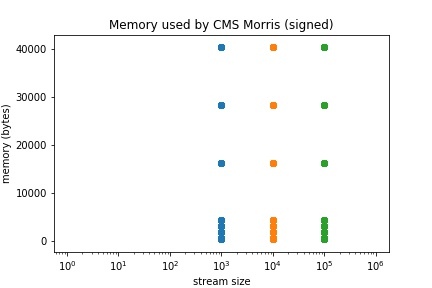
\includegraphics[scale=0.5]{memory_morris_signed}
        \end{center}

        \noindent Comparatively, the memory used by normal hash map is \\

        \begin{center}
            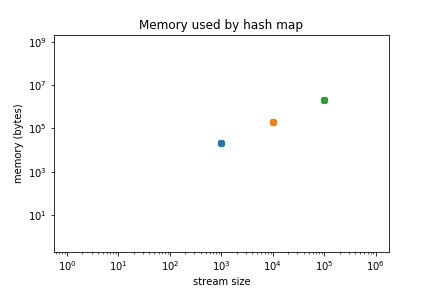
\includegraphics[scale=0.5]{memory}
        \end{center}

        \noindent To get smaller values of $\epsilon$ and $\delta$, the trade of is the increase of space occupied by the counter. Choose the Count-Min Sketch default version as an example.

        \begin{center}
            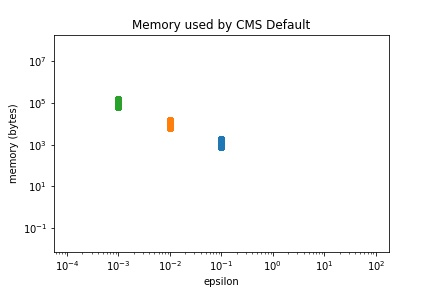
\includegraphics[scale=0.5]{memory_epsilon.jpg}
            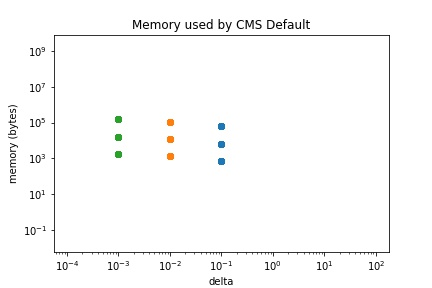
\includegraphics[scale=0.5]{memory_delta.jpg}
        \end{center}

        \noindent These two graphs reflect that $\epsilon$ can affect the size of the counter severely, which is reasonable as $w$ is inverse proportional to $\epsilon$.

        \noindent Another interesting property is the update time of different Count-Min Sketch.

        \begin{center}
            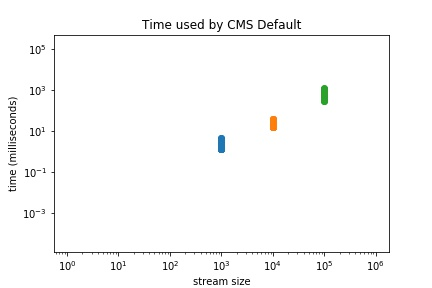
\includegraphics[scale=0.5]{time_default}
            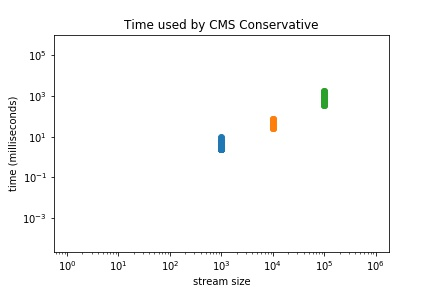
\includegraphics[scale=0.5]{time_conservative}
        \end{center}

        \begin{center}
            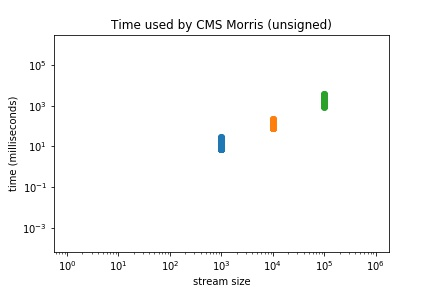
\includegraphics[scale=0.5]{time_morris_unsigned}
            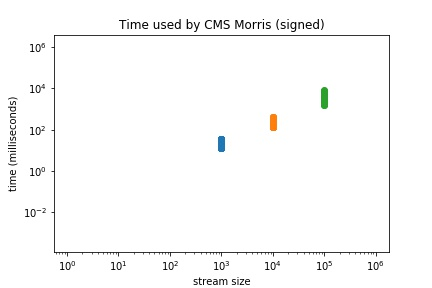
\includegraphics[scale=0.5]{time_morris_signed}
        \end{center}

        \noindent We can see a dramatic increase when the morris counter is used to replace the ordinary counters. From the distribution of the points on the graph, we also can spot that $\epsilon$ and $\delta$ also have slight impact on the update.
    \section{Future Improvement}
        Add more stream generators, such as different distributions and data types, based on the current skeleton can test the Count-Min Sketch more thoroughly. The accuracy model should be replaced by a more effective mechanism instead of strictly following $f_x \leq f_x + \epsilon F_1$.
\end{document}
